\chapter{Stator/Rotor Inerface}
\label{cha:kanal}
Bei der Berechnung des Wirkungsgrades führen geringe Abweichungen der Totaltemperatur zu großen Änderungen des Wirkungsgrades. An dem Stator-Rotor Interface kommt es bei Wahl einer sogenannten Mixing-Plane zur stationären Berechnung zu einem Ansteigen der Totaltemperatur. In diesem Kapitel wird zunächst die Funktionsweise der Mixing Plane erläutert und die Ergebnisse der Analyse des Einflusses der Mixing Plane bei unterschiedlichen Einstrombedingungen vorgestellt.
%______________________________________________________
\section{Mixing Plane / Stage}
In dem verwendeten Setup der Aachenturbine werden die 1,5 Stufen in drei Domänen dargestellt. Hierbei kommt es zu einer Herausforderung; die Domänen müssen miteinander verbunden werden. Um dies zu bewerkstelligen, werden jeweils an den Verbindungsstellen von Stator zu Rotor und Rotor zu Stator sogenannte \textit{Interfaces} definiert.
Im Falle einer solchen Anordnung ist in CFX die \textit{General Connection} zu wählen, da sich rotierende an stationäre Domänen anschließen.\\
Eine Möglichkeit ein solches Interface mittels General Connection zu definieren ist das Frozen Rotor Interface. Hierbei bleibt die relative Orientierung der Komponenten über die gesamte Berechnung erhalten. 
Dieses Modell hat seine Vorteile bei großen Schwankungen der Strömungsgrößen in Umfangsrichtung.\\
Eine weitere Untergruppe der \textit{General Connection} in CFX ist das Stage- oder Mixing Plane-Interface, welches für die Erstellung des in dieser Arbeit verwendeten Setups eingesetzt wird. Hierbei werden die Strömungsgrößen an der Verbindungsstelle über den Umfang gemittelt.
Durch die Mittelung der Strömungsgrößen am Interface treten Vermischungsverluste auf. Laut ANSYS sind die hierbei entstehenden Verluste äquivalent zu den physikalischen Vermischungseffekten der zwischen Stator und Rotor und eines somit entstehenden Geschwindigkeitsprofils in entgegen der Strömungsrichtung. \cite{Sharcnet1}

%_____________________________________________________________________
\section{Rohrauschnitt}
\label{sec:kanalgeo}
Anstelle der Aachen-Turbine wird für die Analyse des Stator-Rotor Interfaces ein Rohrausschnitt, geteilt in Stator und Rotor, berechnet um den Einfluss des Interfaces auf die Strömungsgrößen in Hinblick auf die Wirkungsgradberechnung zu testen. Dabei werden die Eintrittsbedingungen verändert und das Verhalten der Mixing-Plane unter unterschiedlichen Einströmbedingungen untersucht. In dem folgenden Abschnitt wird zunächst das Rechengebiet näher beschrieben.
%________________________________________________________
\subsection{Problemgebiet}
\label{subsec:kanalproblemgebiet}
Die Geometrie des Rohrausschnitts mit Gitter ist in der Abbildung \ref{fig:kanalgebiet} zu sehen.
\begin{figure}[H]
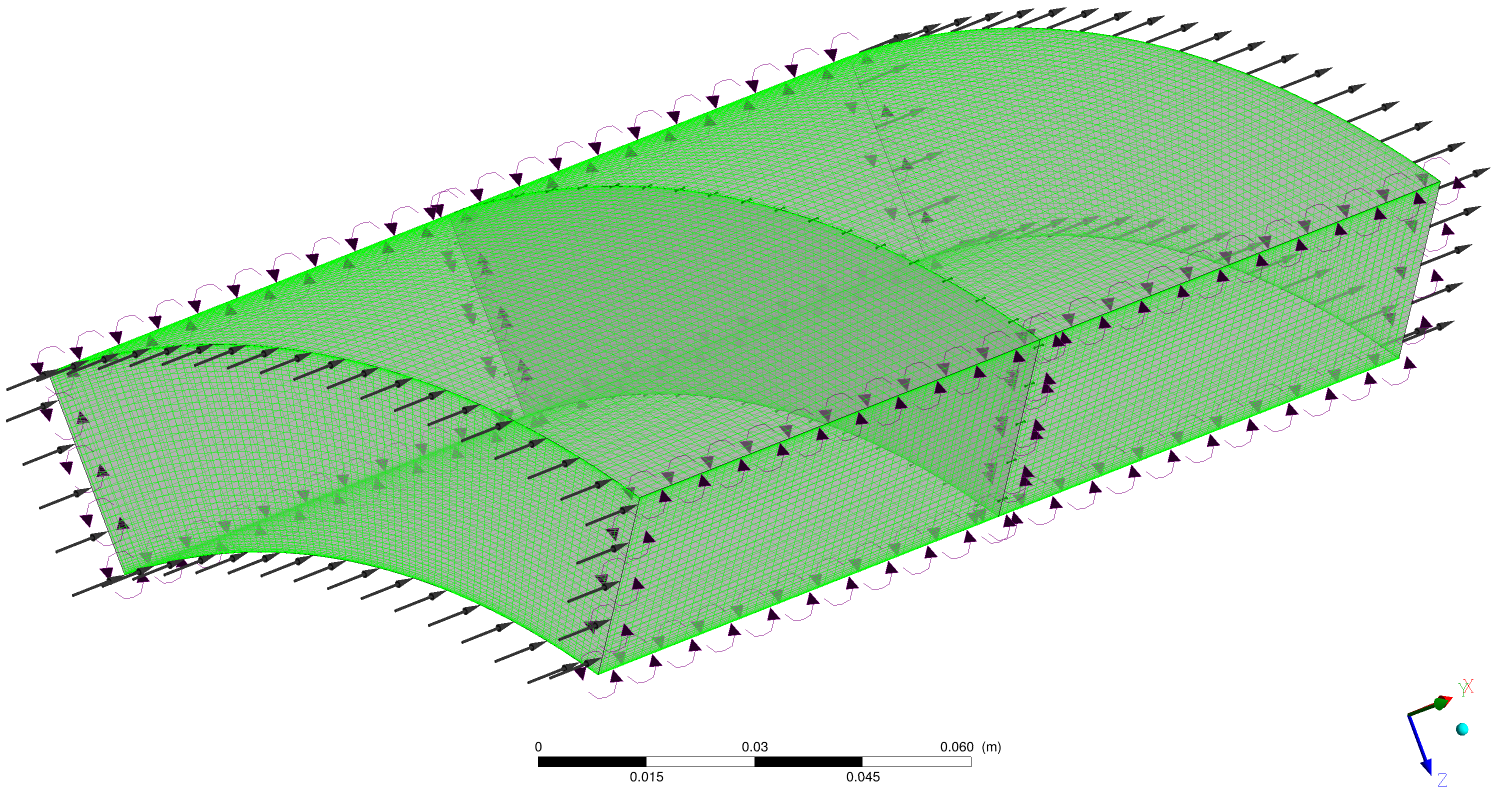
\includegraphics[width=\textwidth]{kanalmitmesh.png}
\caption{Eine dreidimensionale Ansicht der vereinfachten Aachen-Turbine mit Gitter}
\label{fig:kanalgebiet}
\end{figure}
Die vereinfachte Turbine besteht aus einem Stator und einem Rotor. An der Vorderseite befindet sich der Einstrom, an den Seiten jeweils periodische Randbedingungen, an der Rückseite ist der Ausstrom. Die Grenzen an der Ober- und Unterseite stellen Shroud und Hub dar, repräsentieren somit Wandrandbedingungen. Stator und Rotor sind mit einem Interface verbunden. Das Verhältnis der Abmessungen dieses Rohrausschnitts entspricht den Größenverhältnissen der Aachen-Turbine und sind der Tabelle \ref{tab:kanalabmessungen} zu entnehmen.
\begin{table}[H]
\centering
\label{tab:kanalabmessungen}
\caption{Abmessungen der vereinfachten Turbine}
\begin{tabular}{ c| c| c| c}
 $d_a$&$d_i$&$L_x$&$\alpha$\\
\hline
$300mm$&$240mm$&$160mm$&$45^\circ$\\
\end{tabular}
\end{table}
Hierbei sind $d_a$ Außendurchmesser, $d_i$ Innendurchmesser $d_i$, $L_x$ die Länge in Axialrichtung  und $\alpha$ der Ausschnittswinkel.
%________________________________________________________
\subsection{Gitterstudie}
\label{subsec:kanalgitterstudie}
Nach Festlegen der Geometrie wird ein CAD-Modell und ein Gitter mit einem $y^+ \approx 1$ erstellt. Darauf folgte eine Gitterstudie, um die Unabhängigkeit der Lösung zur Gitterdiskretisierung sicherzustellen. Dabei wird das Modell auf immer feiner werdenden Gittern berechnet, bis sich die relevanten Größen nicht mehr verändern. In der folgenden Tabelle \ref{tab:kanalgitter} werden die Gitterparameter des Gitters gezeigt, die aus der Gitterstudie ermittelt und für die Analyse verwendet werden. 
\begin{table}[H]
\centering
\caption{Gitterparameter des Kanals}
\begin{tabular}{ c| c| c| c| c}
$N_x$&$N_r$&$N_\phi$&Gesamtanzahl Knoten&Gesamtanzahl KV\\
\hline
48&56&79 &424704&403260\\
\end{tabular}
\label{tab:kanalgitter}
\end{table}
Dabei sind $N_x$, $N_r$ und $N_\phi$ die Anzahl an Knoten in die verschiedenen Raumrichtungen in Zylinderkoordinaten.\newline
Anschließend werden für dieses Gitter Strömungssimulationen mit unterschiedlichen Eintrittsrandbedingungen und Veränderungen des Stator-Rotor Interfaces durchgeführt, die in dem folgendem Abschnitt beschrieben werden.

%_____________________________________________________________________________
\section{Einfluss des Stator-Rotor Interface auf den Wirkungsgrad}
\label{kanaleinfluss}
In diesem Abschnitt werden die unterschiedlichen verwendeten Eintrittsrandbedingungen näher erläutert und dann die Ergebnisse der verschiedenen Simulationen vorgestellt.
\subsection{Verwendete Eintrittsrandbedingungen}
\label{subsec:kanalrandbedingungen}
Bei dem Stator-Rotor Interface werden die Werte an den Knoten vor dem Interface nach Mittelung und Interpolation auf die Knoten nach dem Interface übertragen. Bei gleichem Gitter für Stator und Rotor können diese direkt zugeordnet werden. Deswegen wird für einen Testfall das Gitter im Rotor verfeinert, sodass die Zuordnung der Knoten interpoliert erfolgen muss.\newline
Des Weiteren wird der Einfluss der Einströmrandbedingung in Bezug auf die Mixing Plane ermittelt. Dabei wird eine schräge Einströmung (Abbildung \ref{fig:randbedingungen}\subref{subfig-2:randbedingungen}), eine inhomogene Temperaturverteilung mit maximaler Temperatur in Rechengebietsmitte (Abbildung \ref{fig:randbedingungen}\subref{subfig-3:randbedingungen}/\subref{subfig-4:randbedingungen}) und schließlich zusätzliche Dralleintrittsrandbedingungen mit unterschiedlicher Drallkernposition (Abbildung \ref{fig:randbedingungen}\subref{subfig-5:randbedingungen}/\subref{subfig-6:randbedingungen}) vorgegeben.
\begin{figure}[htbp]
\centering
%\subfigure[Feineres Gitter im Rotor]{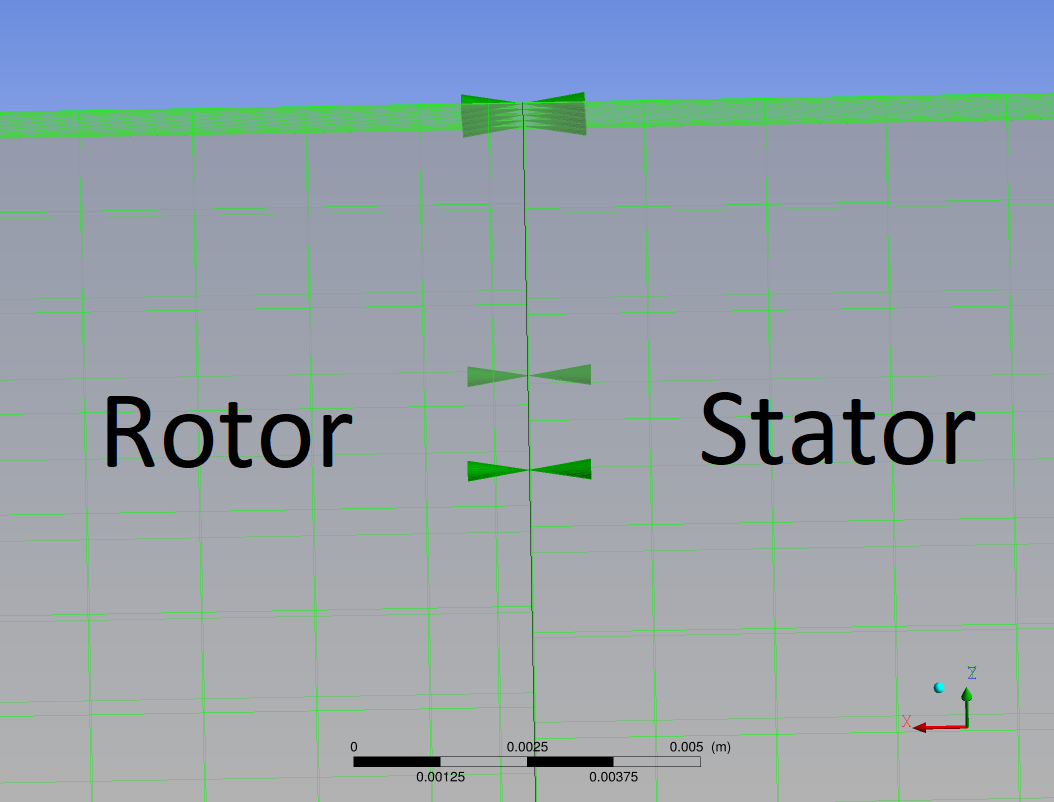
\includegraphics[width=0.45\textwidth]{bilder/feinererrotor.png}\label{subfig-1:randbedingungen}}
\subfigure[Schräger Strömungseintritt]{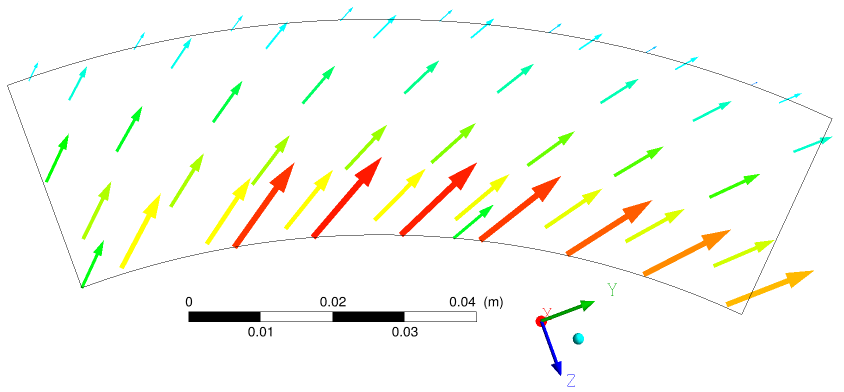
\includegraphics[width=0.8\textwidth]{schraegeStromlinien_Vector.png}\label{subfig-2:randbedingungen}}
\subfigure[Inhomogene $T_t$ (vor Interface)]{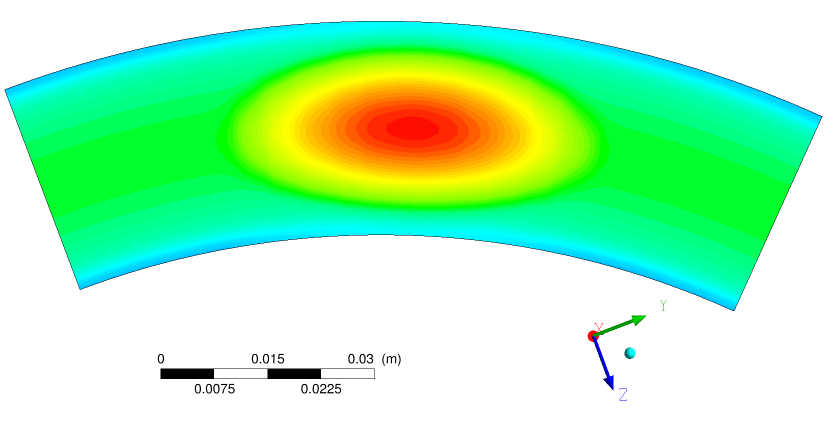
\includegraphics[width=0.45\textwidth]{TtVorMP.png}\label{subfig-3:randbedingungen}}
\subfigure[Inhomogene $T_t$ (nach Interface)]{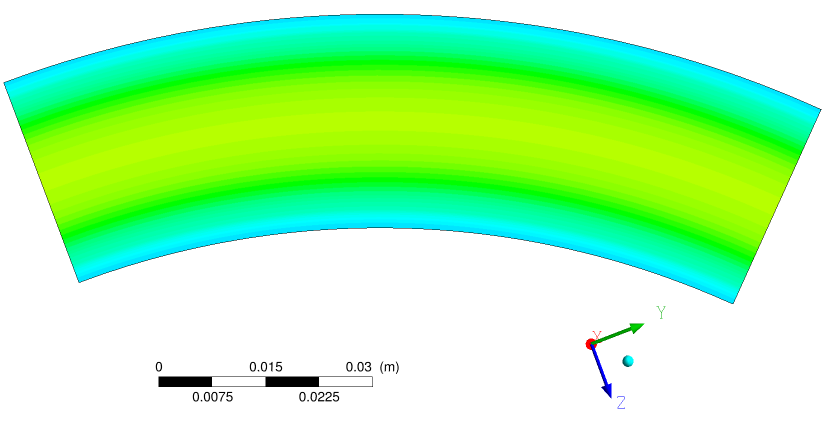
\includegraphics[width=0.45\textwidth]{TtNachMP.png}\label{subfig-4:randbedingungen}}
\subfigure[DralleintrittsRB A]{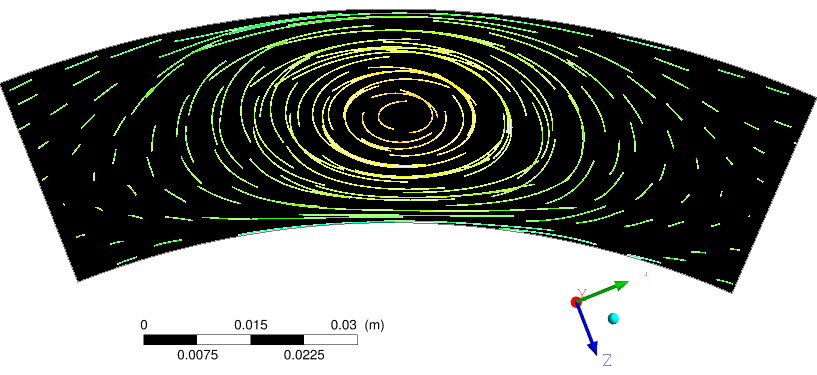
\includegraphics[width=0.45\textwidth]{drallkernA.png}\label{subfig-5:randbedingungen}}
\subfigure[DralleintrittsRB B]{\includegraphics[width=0.45\textwidth]{drallkernb.png}\label{subfig-6:randbedingungen}}
\caption{Verwendete Randbedingungen}
\label{fig:randbedingungen}
\end{figure} 
Anstatt nur stationär mit einer Mixing Plane wurde die Berechnung auch vollständig instationär mit einer Sliding Plane durchgeführt. Die Ergebnisse dieser Berechnungen werden im nächsten Abschnitt vorgestellt.
\subsection{Einfluss auf die Strömungsgrößen}
\label{subsec:einfluss}
Zur Untersuchung des Stator-Rotor Interface sollen die Strömungsgrößen vor und nach dem Interface miteinander verglichen werden. Hierfür werden die Differenz nach
\begin{equation}
\label{eq:tdifferenz}
\Delta T_{t} = T_{t,2} - T_{t,1}
\end{equation}
berechnet, wobei $T_{t,1}$ die Totaltemperatur vor dem Interface und $T_{t,2}$ die Totaltemperatur nach dem Interface ist. Dabei ergibt sich folgende Tabelle \ref{tab:kanalbedingungen} mit den Strömungsgrößen Massenstrom $\dot m$, Totaldruck $p_t$ und Totaltemperatur $T_t$.
\begin{table}[H]
\centering
\caption{Einfluss der Eintrittsrandbedingungen}
\begin{tabular}{ c| c| c| c}
Einstromrandbedingung& $\Delta \dot m$ in $\frac{kg}{s}$ & $\Delta p_t$ in $Pa$ &  $\Delta T_t$ in $K$\\%&$\Delta \eta$\\
\toprule
Referenzlösung&+1,252e-05&-40,04&+0,043\\%&+0,15\%\\
feineres Gitter im Rotor&+3,755e-06&-43,81&+0,043\\%&+0,15\%\\
schräge Einströmung&-7,368e-06&-35,45&+0,026\\%&-0,04\% \\
inhomogene TemperaturRB&+1,078e-06&+10,36&+0,794\\%&+2,29\% \\
DralleintrittsRB A&+9.611e-06&+20.17&+0.012\\%&+5,45\% \\
DralleintrittsRB A + Temperatur RB&-1,051e-05&-38,59&+1,764\\%&+5,45\% \\
DralleintrittsRB B + Temperatur RB&-1,312e-05&-41,83&+1,632\\%&+5,04\% \\
DralleintrittsRB C + Temperatur RB&-8,919e-06&-93,04&+1,719\\%&+5,12\% \\
DralleintrittsRB D + Temperatur RB&-1,539e-05&+2,787&+1,597\\%&+5,11\% \\
DralleintrittsRB E + Temperatur RB&+4,091e-06&-12,07&+1,576\\%&+4,99\% \\
DralleintrittsRB F + Temperatur RB&+1,729e-06&-23,83&+1,626\\%&+5,10\% \\
\midrule
Instationär&+1,873e-07&-0,604&-2,466e-04\\%&+0\% \\
\end{tabular}
\label{tab:kanalbedingungen}
\end{table}
Es ist zu sehen, dass die Massenströme vor und nach dem Stator-Rotor Interface für alle Einstrombedingungen annähernd gleich groß sind. Der Totaldruck sinkt um bis zu maximal $\Delta P_{t_{max}} \approx 93 Pa$, somit ist der Totaldruckverlust im Vergleich zu den vorherrschenden Totaldrücken $\frac{\Delta p_t}{p_t} \approx 10^{-4}$ klein. \newline Die Totaltemperatur ändert sich bei homogenen Temperaturrandbedingungen sowohl für schräge Einströmungsrandbedingungen als auch bei feinerem Gitter im Rotor kaum ($\Delta T_t < 0,05 K$). \newline
Bei inhomogenen Temperaturrandbedingungen unterscheidet sich die Totaltemperatur vor und nach dem Interface um ungefähr $\Delta T_t \approx 0,8K$. Hier ist der Unterschied von $T_t$ im Vergleich zum vorher homogenen Temperaturfeld wesentlich größer. Insbesondere bei zusätzlichen Dralleintrittsbedingungen ergeben sich Totaltemperaturdifferenzen von bis zu $\Delta T_t \approx 1,8K$. Bei Dralleintrittsbedingungen mit inhomogenen Randbedingungen sind somit die Abweichung der Totaltemperatur ungefähr doppelt so hoch wie bei separater inhomogener Temperaturrandbedingung.\\
Die Untersuchung der Mixing Plane erfolgt mit einer vereinfachten Turbine ohne Schaufeln. Bei diesem Fall wird im Rotor ohne Schaufeln keine Leistung erzeugt, sondern der Strömung Energie durch Rotation und Reibung zugeführt. Dies hat zur Folge, dass bei diesem Problemgebiet direkt keine Aussagen über den Wirkungsgrad wie bei einer Turbine getroffen werden kann. Um dennoch zumindest eine grobe Abschätzung der Veränderung des Wirkungsgrades durch die Mixing Plane zu erhalten, werden die Ergebnisse für $\Delta p_t$ und $\Delta T_t$ für diese Geometrie auf die Aachen Turbine übertragen. Dabei wird die Aachen Turbine mit dem gleichen Betriebspunkt wie die vereinfachte Rohrströmung gerechnet und die Differenzen an den beiden Interfaces Stator1-Rotor und Rotor-Stator2 betrachtet. Diese Differenzen werde im nächsten Schritt Wirkungsgradberechnung eliminiert, um einen korrigierten Wirkungsgrad zu erhalten (frei von den Differenzen an der Mixing Plane). Auf diesen korrigierten Wirkungsgrad werden dann die Differenzen, die sich bei der vereinfachten Rohrströmung ergeben haben, wieder aufaddiert, unter der Annahme, dass sich die Aachen Turbine bei unterschiedlichen Eintrittsbedingungen ähnlich wie die Rohrströmung verhält. Damit ergaben sich folgende Abweichungen des Wirkungsgrads $\Delta \eta$ durch die Mixing Plane:
\begin{table}[htbp]
\centering
\caption{Abschätzung des Einflusses der MP auf den Wirkungsgrad}
\begin{tabular}{ c| c}
Einstromrandbedingung&$\Delta \eta$\\
\toprule
Referenzlösung&-0,264\%\\
feineres Gitter im Rotor&-0,274\%\\
schräge Einströmung&-0,190\% \\
inhomogene TemperaturRB&-2,775\% \\
DralleintrittsRB A&-6,345\% \\
DralleintrittsRB B&-5,884\% \\
DralleintrittsRB C&-6,343\% \\
DralleintrittsRB D&-5,629\% \\
DralleintrittsRB E&-5,599\% \\
DralleintrittsRB F&-5,808\% \\
\midrule
Instationär&-8 $\cdot 10^{-4}\%$ \\
\end{tabular}
\label{tab:kanalwg}
\end{table}
Hierbei ist jedoch anzumerken, dass aufgrund der vielen Annahmen diese Abschätzung nicht als allgemeine Aussage für die Wirkungsgradbestimmung zu sehen ist, sondern nur eine grobe Abschätzung der Größenordnung des Einflusses der Mixing Plane darstellt.

\newpage
\subsection{Fazit}
\label{subsec:fazit}
Die Berücksichtung des Einflusses der Mixing Plane für die Wirkungsgradbestimmung ist unerlässlich, sobald inhomogene Temperaturfelder am Interface auftreten oder die Strömung mit kleine Winkeln, das heißt schräg oder mit Drall, auf das Interface auftrifft. Hier sollten die Domänen instationär mit einer Sliding Plane verbunden werden, um die Verfälschung der Strömung durch Mittelung an der Mixing Plane zu vermeiden. Außerdem ist hier zu erwähnen, dass in diesem Testfall nur der Einfluss eines einzelnen Interfaces untersucht wurde. Bei einer Simulationen von mehreren Turbinenstufen und somit der Verwendung von mehreren Interfaces summiert sich der Fehler am Interface.

%%% Local Variables: 
%%% mode: latex
%%% TeX-master: "main"
%%% End: 


